\section{Local\-Tests Class Reference}
\label{classLocalTests}\index{LocalTests@{LocalTests}}
local test of one sync source and utility functions also used by sync tests  


{\tt \#include $<$Client\-Test.h$>$}

Collaboration diagram for Local\-Tests:\begin{figure}[H]
\begin{center}
\leavevmode
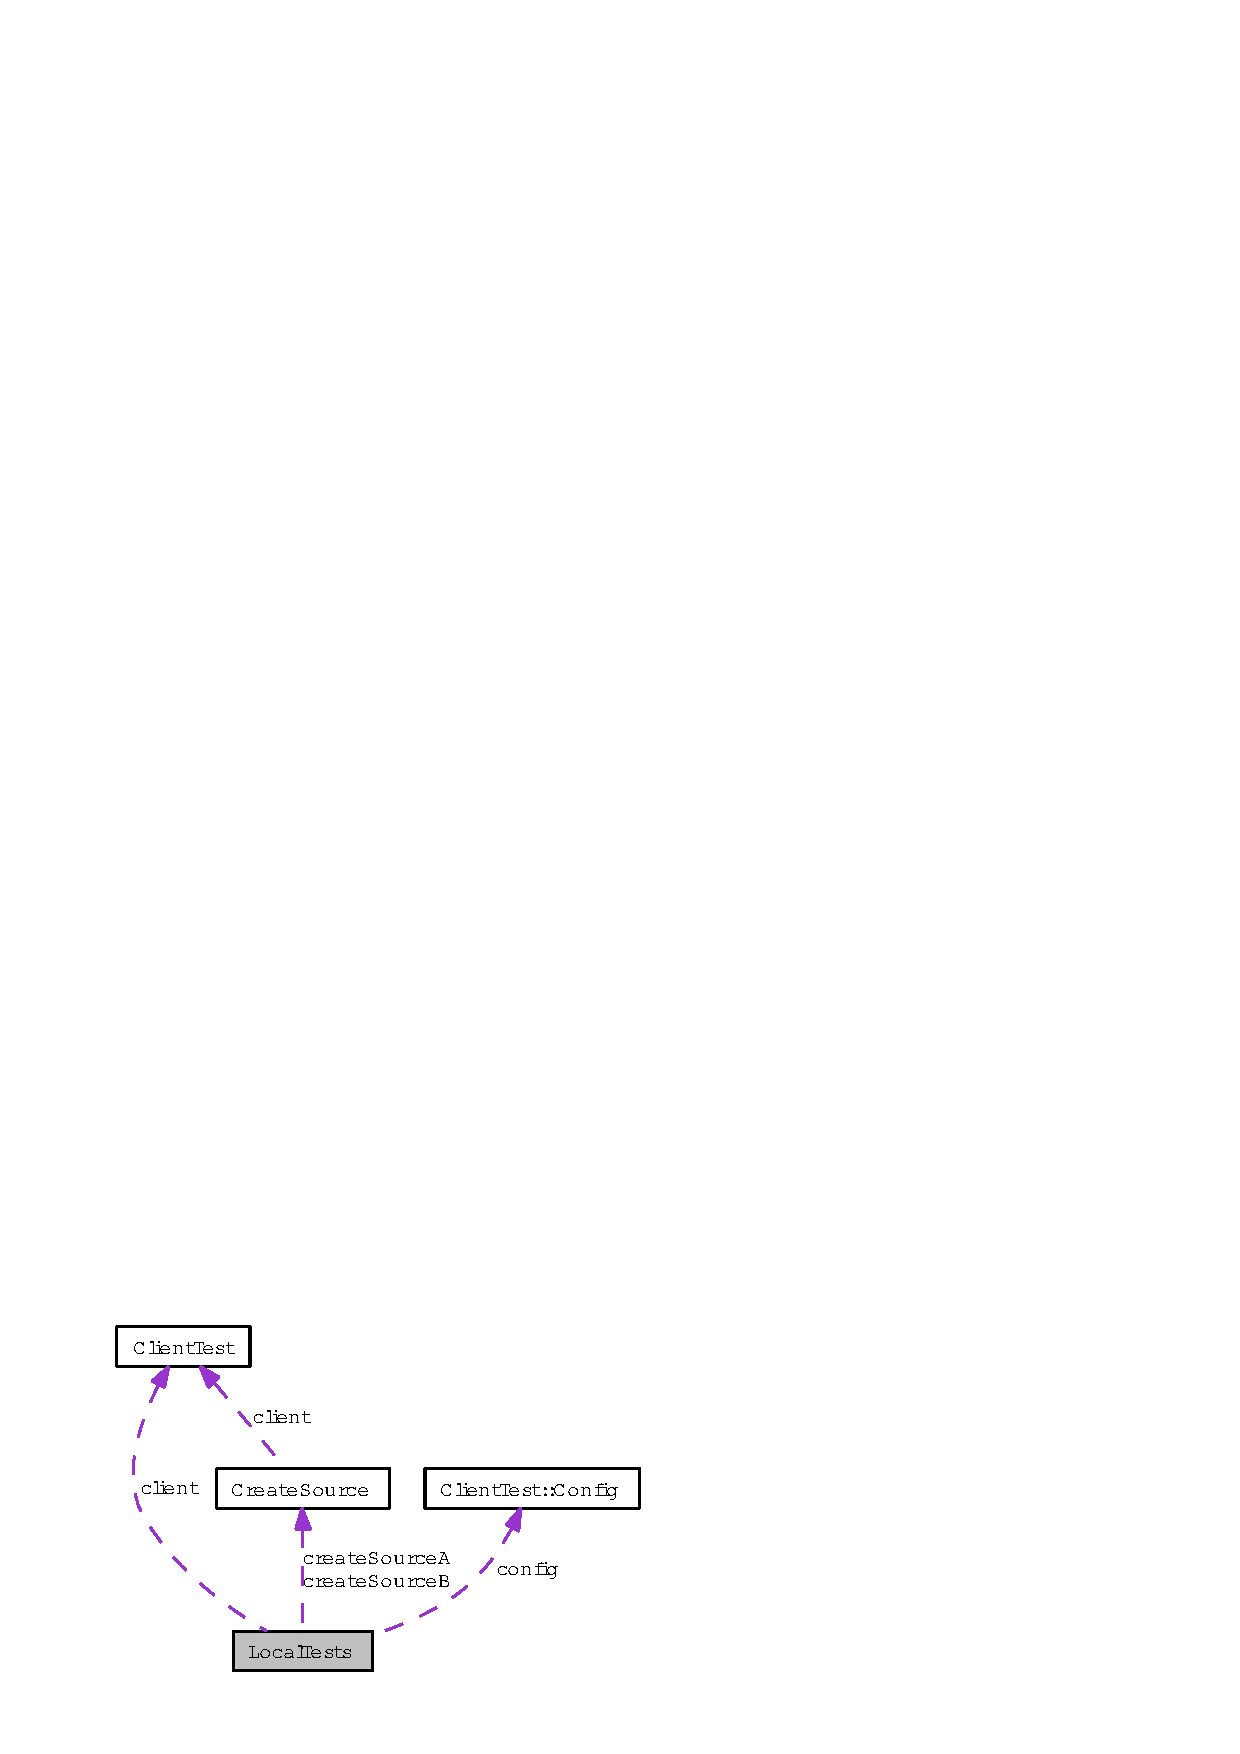
\includegraphics[width=155pt]{classLocalTests__coll__graph}
\end{center}
\end{figure}
\subsection*{Public Member Functions}
\begin{CompactItemize}
\item 
\textbf{Local\-Tests} (const std::string \&name, {\bf Client\-Test} \&cl, int source\-Param, {\bf Client\-Test::Config} \&co)\label{classLocalTests_d20120d9d597a0e81bdaf4651a7c04e7}

\item 
virtual void {\bf add\-Tests} ()\label{group__ClientTest_ga75ca0b749c031d14d99f11ad72fa3dd}

\begin{CompactList}\small\item\em adds the supported tests to the instance itself; this is the function that a derived class can override to add additional tests \item\end{CompactList}\item 
virtual std::string {\bf insert} ({\bf Create\-Source} create\-Source, const char $\ast$data, bool relaxed=false)
\begin{CompactList}\small\item\em opens source and inserts the given item; can be called regardless whether the data source already contains items or not \item\end{CompactList}\item 
virtual void {\bf update} ({\bf Create\-Source} create\-Source, const char $\ast$data, bool check=true)
\begin{CompactList}\small\item\em assumes that exactly one element is currently inserted and updates it with the given item \item\end{CompactList}\item 
virtual void {\bf delete\-All} ({\bf Create\-Source} create\-Source)\label{group__ClientTest_g85fef3b837faa5952472285c0f460faf}

\begin{CompactList}\small\item\em deletes all items locally via sync source \item\end{CompactList}\item 
virtual void {\bf compare\-Databases} (const char $\ast$ref\-File, {\bf Sync\-Source} \&copy, bool raise\-Assert=true)
\begin{CompactList}\small\item\em takes two databases, exports them, then compares them using synccompare \item\end{CompactList}\item 
virtual int {\bf insert\-Many\-Items} ({\bf Create\-Source} create\-Source, int start\-Index=1, int num\-Items=0, int size=-1)
\begin{CompactList}\small\item\em insert artificial items, number of them determined by TEST\_\-EVOLUTION\_\-NUM\_\-ITEMS unless passed explicitly \item\end{CompactList}\item 
virtual void \textbf{test\-Open} ()\label{group__ClientTest_g86523e51eeb7f4b2f9af40483952a13d}

\item 
virtual void \textbf{test\-Iterate\-Twice} ()\label{group__ClientTest_ge859169c3e1f1306be4b7fdb74635c08}

\item 
virtual void \textbf{test\-Simple\-Insert} ()\label{group__ClientTest_g4f6150f962c87e26e04462237471eb59}

\item 
virtual void \textbf{test\-Local\-Delete\-All} ()\label{group__ClientTest_g51dc0792ddba8ef6edafa0cf14b9e0fa}

\item 
virtual void \textbf{test\-Complex\-Insert} ()\label{group__ClientTest_g33765a5f9ea2b98b9f5db89e45275603}

\item 
virtual void \textbf{test\-Local\-Update} ()\label{group__ClientTest_gfe4acc8d97f4c4511b07f1283254aecc}

\item 
virtual void \textbf{test\-Changes} ()\label{group__ClientTest_g9eafd5c7f66ec1a01130fe906bf4fbf4}

\item 
virtual void \textbf{test\-Import} ()\label{group__ClientTest_g18af29fdc3e8816478d535fc80809ed2}

\item 
virtual void \textbf{test\-Import\-Delete} ()\label{group__ClientTest_g1f87c00619bf71f26ae9a7a35e410803}

\item 
virtual void \textbf{test\-Many\-Changes} ()\label{group__ClientTest_gc79d3081b27df1fd5c12070a23f7dc0f}

\item 
virtual void \textbf{test\-Linked\-Items\-Parent} ()\label{group__ClientTest_g8265afa4aecbf4e83018e0f548240f78}

\item 
virtual void \textbf{test\-Linked\-Items\-Child} ()\label{group__ClientTest_g3a1ceae09c7df3f02f6f53eb881cb6c6}

\item 
virtual void \textbf{test\-Linked\-Items\-Parent\-Child} ()\label{group__ClientTest_g354b51e8adb792f812f055833f19d646}

\item 
virtual void \textbf{test\-Linked\-Items\-Child\-Parent} ()\label{group__ClientTest_g4584aad53aa76ed65407f11b688728bf}

\item 
virtual void \textbf{test\-Linked\-Items\-Child\-Changes\-Parent} ()\label{group__ClientTest_g4fb2e1ea39ad207556b9ce3e2f2de7a1}

\item 
virtual void \textbf{test\-Linked\-Items\-Remove\-Parent\-First} ()\label{group__ClientTest_g45620d674aa31cc534509c7064da284d}

\item 
virtual void \textbf{test\-Linked\-Items\-Remove\-Normal} ()\label{group__ClientTest_g9ddb7acaef74dbb7bc27422c5b74181f}

\item 
virtual void \textbf{test\-Linked\-Items\-Insert\-Parent\-Twice} ()\label{group__ClientTest_g2e2b4217c211ea719388105619d45a60}

\item 
virtual void \textbf{test\-Linked\-Items\-Insert\-Child\-Twice} ()\label{group__ClientTest_g6ee12660ef78fad16d27748ff20d8183}

\item 
virtual void \textbf{test\-Linked\-Items\-Parent\-Update} ()\label{group__ClientTest_ge05a18788fbdd8360b4a10721036beb7}

\item 
virtual void \textbf{test\-Linked\-Items\-Update\-Child} ()\label{group__ClientTest_g530727d8122c69b8008be62652af7755}

\item 
virtual void \textbf{test\-Linked\-Items\-Insert\-Both\-Update\-Child} ()\label{group__ClientTest_g5d0e06ba1cac19805ec0d7d0dfbe21e7}

\item 
virtual void \textbf{test\-Linked\-Items\-Insert\-Both\-Update\-Parent} ()\label{group__ClientTest_g7eab80ca6d905dffba6552f8a965fe1d}

\end{CompactItemize}
\subsection*{Public Attributes}
\begin{CompactItemize}
\item 
{\bf Client\-Test} \& {\bf client}\label{classLocalTests_e5709a00bd1d0c0aaa98c48ed255098c}

\begin{CompactList}\small\item\em the client we are testing \item\end{CompactList}\item 
const int {\bf source}\label{classLocalTests_08ad8ca8670698be655bf547a78b4471}

\begin{CompactList}\small\item\em number of the source we are testing in that client \item\end{CompactList}\item 
const {\bf Client\-Test::Config} {\bf config}\label{classLocalTests_b745c9235176e04fae5a0b918aebb87e}

\begin{CompactList}\small\item\em configuration that corresponds to source \item\end{CompactList}\item 
{\bf Create\-Source} {\bf create\-Source\-A}\label{classLocalTests_a3e9f028a40fbe46322ac2e7e8fe5640}

\begin{CompactList}\small\item\em helper funclets to create sources \item\end{CompactList}\item 
{\bf Create\-Source} \textbf{create\-Source\-B}\label{classLocalTests_abae458e7851e1dbc05eba556037a5ed}

\end{CompactItemize}


\subsection{Detailed Description}
local test of one sync source and utility functions also used by sync tests 



The documentation for this class was generated from the following files:\begin{CompactItemize}
\item 
test/Client\-Test.h\item 
test/Client\-Test.cpp\end{CompactItemize}
